\documentclass[tikz,border=3pt]{standalone}
\usepackage[utf8]{inputenc}
\usepackage[T1]{fontenc}
\usepackage{lmodern}
\renewcommand{\familydefault}{\sfdefault}
\usepackage{sansmath}\sansmath
\usepackage{chemfig}
\usepackage{pgfplots}\pgfplotsset{compat=1.18,/pgf/number format/use comma,/pgf/number format/1000 sep={.}}
\usetikzlibrary{arrows.meta,calc,positioning,decorations.pathmorphing,patterns}
% paleta del sitio
\definecolor{nar}{HTML}{E8680C}\definecolor{narc}{HTML}{FFB35C}\definecolor{hielo}{HTML}{FFF3E8}
\definecolor{tinta}{HTML}{1D1D1F}\definecolor{gris}{HTML}{6E6E73}\definecolor{lila}{HTML}{7C5CF0}
\definecolor{azul}{HTML}{2F6FD6}\definecolor{menta}{HTML}{17A673}\definecolor{coral}{HTML}{E8342A}
\begin{document}
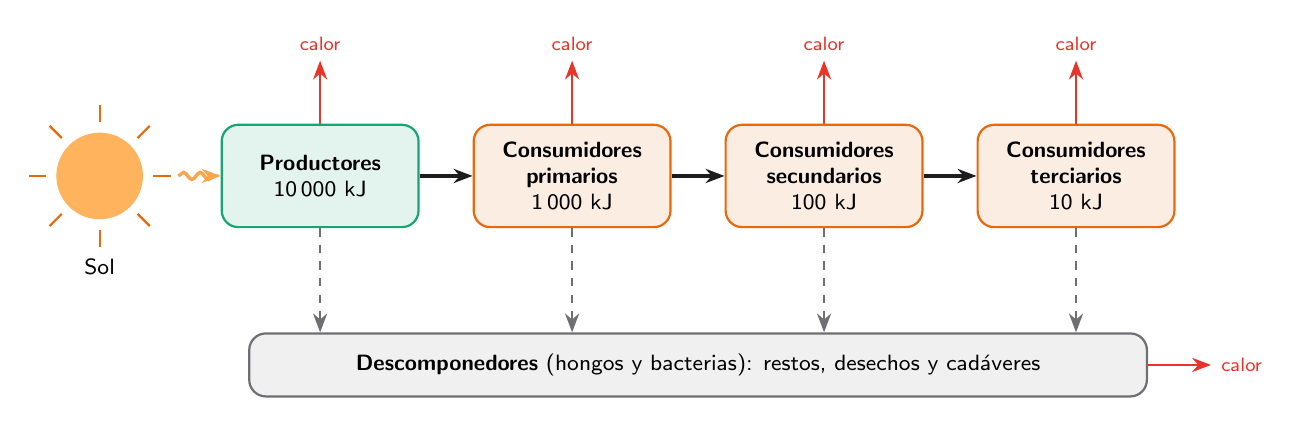
\begin{tikzpicture}[font=\small,>={Stealth[length=2.4mm]}]
\tikzset{niv/.style={draw=#1,fill=#1!12,thick,rounded corners=6pt,minimum width=2.5cm,minimum height=1.3cm,align=center,font=\footnotesize}}
\fill[narc] (-0.4,0) circle (0.55); \foreach \a in {0,45,...,315} \draw[nar,thick] ($(-0.4,0)+(\a:0.68)$) -- ($(-0.4,0)+(\a:0.9)$);
\node[font=\footnotesize] at (-0.4,-1.15) {Sol};
\node[niv=menta] (P) at (2.4,0) {\textbf{Productores}\\10\,000 kJ};
\node[niv=nar] (C1) at (5.6,0) {\textbf{Consumidores}\\\textbf{primarios}\\1\,000 kJ};
\node[niv=nar] (C2) at (8.8,0) {\textbf{Consumidores}\\\textbf{secundarios}\\100 kJ};
\node[niv=nar] (C3) at (12.0,0) {\textbf{Consumidores}\\\textbf{terciarios}\\10 kJ};
\draw[->,very thick,narc!80!nar,decorate,decoration={snake,amplitude=1.3pt,segment length=6pt}] (0.6,0) -- (P.west);
\draw[->,very thick,tinta] (P) -- (C1); \draw[->,very thick,tinta] (C1) -- (C2); \draw[->,very thick,tinta] (C2) -- (C3);
\foreach \n in {P,C1,C2,C3} \draw[->,thick,coral] (\n.north) -- ++(0,0.8) node[anchor=south,font=\scriptsize,text=coral] {calor};
\node[draw=gris,fill=gris!10,thick,rounded corners=6pt,minimum width=11.4cm,minimum height=0.8cm,font=\footnotesize] (D) at (7.2,-2.4) {\textbf{Descomponedores} (hongos y bacterias): restos, desechos y cadáveres};
\foreach \n in {P,C1,C2,C3} \draw[->,thick,gris,dashed] (\n.south) -- (\n.south |- D.north);
\draw[->,thick,coral] (D.east) -- ++(0.8,0) node[anchor=west,font=\scriptsize,text=coral] {calor};
\end{tikzpicture}
\end{document}
